\documentclass[a4paper, oneside, 11pt]{article}
\usepackage[utf8]{inputenc}
\usepackage[left=2cm,right=2cm,top=2cm,bottom=2cm]{geometry}
\usepackage{longtable}
\usepackage{graphicx}
\usepackage{tikz}
\usepackage{mathtools}
\usepackage{amsmath}
\usepackage{pgfplots}
\usetikzlibrary{plotmarks}
\usepackage{float}
\usepackage{caption}
\usepackage{subcaption}
\usepackage{hyperref}
\usepackage{amssymb}
\usepackage{booktabs}
\usepackage{scrextend}
\usepackage{siunitx}
\usepackage{multirow}

%% WORK DIVISION
%% Trajectory analysis: Julie, Alexandre, Kostas
%% ADCS: Federico, Francesco
%% Telemetry: Camil
%% Payload: Ramin, Bill
%% Solar panels (power system); eclipse duration, power dependency from the distance from the Sun: Simo, Mathias
%% Propulsion system: Simo, Kostas, Yue
%% Thermal design (Surface properties, active heaters, other thermal elements): Group B
%% Batteries and other parts of the power system: Group A + Mathias + Camil

\title{\Huge{Spacecraft Design Study} \\ GROUP AB}
\author{A. Cisowski, R. Farid, F. Giuliano, J. Imbert, Y. Jiao,\\ C. Muresan, M. Nicolle, K. Papavramidis, S. Simolin, F. Raiti\\}
\date{\today}



\begin{document}

\maketitle

\clearpage

\tableofcontents

\clearpage 

%\listoffigures


\section{Introduction}
 
The purpose of this report is to design a spacecraft mission to Mars, with focus on the power and thermal systems. The goal of the mission is to conduct a photographic survey of the Martian surface using a camera with a resolution of 400x400 pixels, which images a surface area of 200x200 km. The total mission duration is 3 years, taking the spacecraft from lower Earth orbit to a Mars polar orbit, where it will image the surface of the planet. The required thermal environment inside the satellite is -20 to +40 $^{\circ}C$ during operation, and -50 to +80 $^{\circ}C$ when the camera is turned off. \\
  

\section{Mission analysis}

A Oberth transfer is used to reach Mars starting from Low Earth Orbit (LEO), with an inclination change operated when arriving at Mars.
The whole trajectory needs two burns. One to go from LEO to Mars on an elliptic trajectory and the other one to leave the ellipse and enter into a Low Mars orbit (LMO).\\
The data used for the calculations of the total $\Delta v$ needed to reach orbit around Mars are detailed in Table \ref{data}. In this table, $M_x$ are the masses, $r_x$ are the radius of orbits around the sun, $r_{LEO}$ is the radius of the low Earth orbit, $r_{LMO}$ is the radius of the low Mars orbit, $\mu_{X}=G*M_x$ and finally the distance between the Sun and the half-point between Earth and Mars.

\noindent After launch, the spacecraft is assumed to be placed on a low circular Earth orbit (LEO) at an altitude of 300 km. 

\begin{table}[!h]
 \caption{Numerical data for the calculations of the $\Delta v$}
 \label{data}
\centering
 \begin{tabular}{| c | c |c |c |c | c|}
  \hline
 $M_{earth}$ & $M_{sun}$ & $M_{mars}$ & $r_{E}$ & $r_{M}$ & $r_{LEO}$ \\
     \hline
  $5.975*10^{24}$ kg & $1.989*10^{30}$ kg & $6.387*10^{23}$ kg & $149.5*10^9$ m& $227.8*10^9$ m & $6.67123*10^6$ m\\
     \hline
\end{tabular}
\end{table}

$
\begin{array}{lr}
g_{0}=\SI{9.81}{m/s^{2}}  \\
\end{array}
$

\begin{table}[!h]
\centering
 \begin{tabular}{| c | c| c|c|}
  \hline
  $r_{LMO}$ &  G & $\mu_{E}$ & $\mu_{S}$  \\
     \hline
 $3.932153*10^6$ m & $6.67*10^{-11} \ \SI{}{m^{3}.kg^{-1}.s^{-2}}$ & $3.985*10^{14} \ \SI{}{m^{3}.s^{-2}}$ & $1.326*10^{20} \ \SI{}{m^{3}.s^{-2}} $ \\
     \hline
\end{tabular}
\end{table}

\begin{table}[!h]
\centering
 \begin{tabular}{|c|c|}
  \hline
 $\mu_{M}$ & a \\
     \hline
 $4.26*10^{13} \ \SI{}{m^{3}.s^{-2}}$ & $1.886*10^{11}$ m\\
     \hline
\end{tabular}
\end{table}

The velocities of the satellite on a circular orbit around a planet is given by equation  a planet is given a $v = \sqrt{ \mu_x / r_x }$.

\noindent This equation gives a velocity $v_{LEO}=7.7$  $\SI{}{km.s^{-1}}$ at 300~km and $v_{LMO}=3.3 $ $\SI{}{km.s^{-1}}$ at 600~km for Mars.

\medskip
\noindent An optimization of the Hohmann transfer is used, called Oberth transfer, which allows to reach Mars from Earth \cite{MechanicsBook}. 
It consists of:
\begin{itemize}
\item Thrusting from LEO to transfer orbit to Mars
\item Thrusting from transfer orbit to Mars orbit.
\end{itemize}

\noindent Considering that the aim of the launch is Mars observation, a polar orbit at 600 km will allow to cover the whole surface of the planet. A change of orbit plane is then necessary from equatorial plane to polar orbit. The inclination change starts as soon as the satellite enters the MTO, where the distance is the biggest at that point, thus the velocity is smaller compared to that one close to Mars and the $\Delta v$ needed for this maneuver is considered very small compared to the ones needed for the other transfers and it is neglected in the following calculations. 

\medskip

\underline{Thrust from LEO to MTO}

\medskip

This transfer includes several steps done at the same time, including:
\begin{itemize}
\item Thrusting from LEO to Earth's SOI.
\item Thrusting from Earth's SOI to MTO.
\end{itemize}

The velocity of the spacecraft on the transfer orbit at the Earth level is given by Equation \ref{vOE}.
 
\begin{equation}
\label{vOE}
\fbox{$V_{T1}=\sqrt{\frac{2*\mu_S}{r_E}-\frac{\mu_S}{a}}$}
\end{equation}

The velocity of the Earth around the sun is given by Equation \ref{vE}. 

\begin{equation}
\label{vE}
\fbox{$v_{earth}= \sqrt{\frac{\mu_S}{r_{E}}}$}
\end{equation}

The escape velocity of the spacecraft from LEO is given by Equation \ref{esc}.

\begin{equation}
\label{esc}
\fbox{$v_{esc_{LEO}}= \sqrt{\frac{2*\mu_E}{r_{LEO}}}$}
\end{equation}

Finally the $\Delta v_1$ necessary to reach the transfer orbit to Mars from LEO is given by Equation \ref{deltavV1}.

\begin{equation}
\label{deltavV1}
\fbox{$\Delta v_1= \sqrt{v_{esc_{LEO}}^2+(v_{T1}-v_{earth})^2}-v_{LEO}$}
\end{equation}

The numerical results for this first $\Delta v_1$ are given in Table \ref{deltaV1Tab}.

\begin{table}[!h]
 \caption{Numerical results from LEO to transfer orbit.}
 \label{deltaV1Tab}
\centering
 \begin{tabular}{| c | c |c |c |}
  \hline
 $v_{esc_{LEO}}$ & $v_{T1}$ & $v_{Earth}$ &  $\Delta v1$  \\
     \hline
  $ 1.093*10^4 \SI{}{m.s^{-1}}$  & $ 3.2723*10^4 \SI{}{m.s^{-1}}$ & $ 2.9781*10^4 \SI{}{m.s^{-1}}$ & $ 3.591*10^3 \SI{}{m.s^{-1}}$ \\
     \hline
\end{tabular}
\end{table}

\underline{Thrust from MTO to LMO}

\medskip
\noindent The $\Delta v_2$ necessary to go from transfer orbit to the final orbit around Mars can be calculated with the same equations as previously. 

\noindent The numerical results for this second $\Delta v_2$ are given in Table \ref{deltaV2Tab}.

\begin{table}[!h]
 \caption{Numerical results from transfer orbit to final orbit around Mars.}
 \label{deltaV2Tab}
\centering
 \begin{tabular}{| c | c |c |c |}
  \hline
 $v_{esc_{LMO}}$ & $v_{T2}$ & $v_{Mars}$ &  $\Delta v2$  \\
     \hline
  $ 4.654*10^3 \SI{}{m.s^{-1}}$  & $ 2.1473*10^4 \SI{}{m.s^{-1}}$ & $ 2.4126*10^4 \SI{}{m.s^{-1}}$ & $ 2.0655*10^3 \SI{}{m.s^{-1}}$ \\
     \hline
\end{tabular}
\end{table}

\medskip

\noindent In the end this trajectory recquires $\Delta v_{total}= 5.6565 *10^3 \ \SI{}{m.s^{-1}}$.

\medskip

\underline{Time of travel}

\medskip

\noindent Assuming that the satellite  reaches Mars in half distance of the elliptical transfer orbit, the travel time is given as $P^2= \frac{4*\pi^2*a^3}{\mu_S}$, resulting in approximatively 8.6 months of travel between Earth and Mars.

\section{Spacecraft design}

\subsection{AOCS}

The attitude and orbit control system (AOCS) is intended to stabilize the satellite along its three axis. It relies on 2 star trackers, 4 sun sensors, IMU and 4 Reaction wheels. In addition, 8 supplementary thrusters are used to reinforce the control. The ACS secondary objective is to allow the spacecraft to assume different configurations during the phases of the flight, namely the detumbling, the cruise and the orbital phase. \\
Here it is important to say that the attitude of each payload component has not been taken into account, i.e. the orientation of the gimbal of the solar panels is not included in the ACS, while the influence of external disturbances, like the solar wind hitting the panels, are embodied in the control algorithm. \\

\subsubsection{Assumptions}

The requirement for this mission is to have enough accuracy to allow the satellite antenna to point the earth, during Mars orbit. For orbit propagation and estimation one-way Doppler effect combined with Kalman filtering will make the estimation strategy for the orbit. Data from star trackers and sun sensors will be considered enough to satisfy the accuracy requirement. \\

\subsubsection{Sensors}

For attitude estimation, 2 star trackers have been chosen as the main sensors because of their high accuracy. Star trackers have full autonomy in attitude acquisition and update. However, they are really sensitive to sunlight, from which they can be damaged in case of direct exposure. For this reason, 6 coarse sun sensors are required to improve the robustness of the system.\\
Two sun sensors will be placed on the same side of the solar panels, as an indicator of sunlight.

An IMU is used to keep track of the spacecraft motion. It contains a gyroscope, an accelerometer and a magnetometer. Data will be reconstructed and stored on-board until a communication window is available, where they will be transmitted through the telemetry channel. The reconstruction process will end saving attitude information as quaternions. Eventually, the attitude will be included in a Kalman filter in order to estimate and evaluate the orbit propagation.

% Power dissipation Terma HE-5AS (https://www.terma.com/media/101677/star_tracker_he-5as.pdf) = 3x7 W
% Coarse sun sensors (http://www.moog.com/literature/Space_Defense/Spacecraft/AOCS-GNC/Coarse_Sun_Sensor.pdf) no power input needed and negligible power dissipation.

\subsubsection{Attitude control and further problems}

Four Reaction wheels are used for attitude control, 3 positioned along the main three axis and one is placed for redundancy. Moreover, eight thrusters for attitude control are used to help the Reaction Wheel(RW) both performing angular momentum desaturation (AMD) and maintaining the attitude while exiting the cruise phase.\\
Three main control modes has been evaluated for this mission: Sun Pointing Mode (SPM), namely the configuration after detumbling and for cruise phase, Mission Mode (MM), which is the nominal attitude the satellite shall have during Mars orbit with camera pointing the planet, Safe Mode (SM), used if both of the star trackers or one RW are down. In this latter mode the satellite shall use only the sun sensor to determine the attitude when in sunlight and keep the attitude before going in eclipse, then, when sun sensors are available again, the RW and the thrusters (if needed) can change the attitude.\\
The spacecraft during cruise, and during orbit around mars, encounters external torque that can influence its attitude and saturate the Reaction wheels, especially the problems regarding Solar pressure, Outgassing phenomena and thruster calibration. The latter is less intuitive with respect the other two. Actually, the ACS thruster are paired in a way that the total $\delta V$ is zero. However small misalignment can occur and in-orbit calibration is demanded before starting operations. \\ 
AMD will be done weekly when the angular momentum of at least one reaction wheel will reach approximately 60\% of maximum value. It will be achieved by means of ACS thrusters.

\subsection{Payload}

\subsubsection{Camera}
The camera that is provided for the mission has the following specifications: 5 kg of mass, 5W of power consumption when turned on, and a resolution of 500 m per pixel that covers a 200 by 200 km area of the Martian surface. This directly translates to an image size of 400x400 pixels, weighing $1250$ kB as each pixel contains 8 bits of data.

\subsubsection{Image data size}This part is an analysis of the data size of the images and therefore the bitrate needed to transmit them to Earth. For this part we will assume that the satellite is always taking pictures regardless of the lighting of the surface and that the satellite stays in the equatorial plane. This gives us the theoretical worst case as it implies sending the most data per time unit.\\
The area covered by the satellite orbiting Mars is a circular sector.
The satellite is in a circular orbit at an altitude of 600 km above the surface, which corresponds to an orbital velocity of 3.27 km/s. The angular orbit velocity around mars is then: $\omega_{mars}=0.00082\quad rad/s$. The ground speed is :  $V_{mars}=\omega_{mars} R_{mars}cos(\theta) = 2.78 \ km/s$. In our case $\theta = 0$ as it is assumed that the satellite stays in the equatorial plane. In reality $\theta$ changes but it only reduces the ground speed which is not going to be the limitating factor in terms of data transfer rates.  For the camera to cover the entire surface, it has to take a picture for every 200 km of the Martian surface, which is every 72 seconds. However  some overlapping has to be introduced to make the fitting of the images together easier, therefore the camera will take a picture every 31 seconds. This represents 247 pictures per orbit.\\
The initial size of a picture is $1250$ kb, assuming each pixel contains 8 bits of data. This image can the be saved and compressed as a jpeg file, with a compression ratio of typically 3:1. The compression can be done by the on board calculator, making the sizes of the compressed jpeg images to be transmitted: $417$ kb. The data amount per orbit is therefore 100,7 MB  for this compression ratio. The maximum data amount to be transfered to Earth during the mission is of 927 GB. Taking into account the fact that in reality the camera will not take pictures while it is in the shadow part of Mars, the actual data amount will be closer to 811 GB.

\subsubsection{Telemetry}
The telecommunication system retained is the  Electra Transceiver from \cite{Electra}. It has a  mass of 4.9kg, and Using a 0.5m X-band antenna it can send informations to earth at a speed of 8192.0 kbps. At maximum usage, it consumes up to 68W of power. Transferring the maximum amount of 100.7 MB data for each orbit takes 12.6 seconds for this system, which can be achieved as the time window for which the satellite has visibility on earth is much bigger ( \~ 5000 s). 

\subsection{Power System}
The purpose of the power system of the spacecraft is to provide electrical power for the payload and for subsystems supporting it, including transmitter sending images back to Earth. Sufficient amount of power shall be delivered in all conditions during the mission; in transfer orbit from Earth to Mars and in orbit around Mars both in eclipse and in sunlight.\\
The structure of the power system is shown in Figure \ref{picture_power_system_diagram}. All the components shown in this graph are listed next and described briefly. Solar arrays and batteries are discussed more thoroughly later in this chapter. 

\begin{itemize}
\item \textbf{Solar array (i.e. solar panels):} Primary power source of the spacecraft. Converts solar irradiance to electric power through photovoltaic effect. Can produce power only when in sunlight.
\item \textbf{Batteries:} Secondary power source of the spacecraft. Provides power by discharging itself when solar panels are not active.
\item \textbf{Shunt voltage limiter:} If solar array produces excess power this excess power is discharged through shunt voltage limiter. This maintains steady voltage output from the solar array. \cite{Shunt voltage limiter}
\item \textbf{Charge control:} During battery charging, a charge controller makes sure that the battery is not overcharged and that the charging happens in tolerable current level
\item \textbf{Discharge by-pass:} If there is a need to discharge the battery for maintenance purposes it is done through discharge by pass in a controlled manner with a current rate that does not harm the battery
\item \textbf{Regulation:} Regulates the voltage supplied for the load keeping the voltage at steady constant level.
\end{itemize}

\begin{figure}[H]
	\centering 
	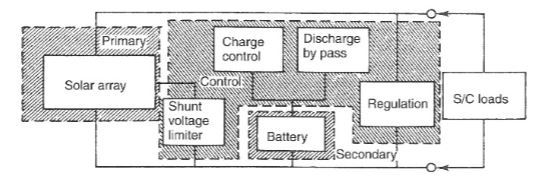
\includegraphics[width=0.7\textwidth]
    {Pictures/power_system_diagram.JPG}
    \caption{Diagram of the spacecraft power system \cite{Power Systems Lecture EF2260}}
    \label{picture_power_system_diagram}
\end{figure}

\subsubsection{Power budget}

Before designing the primary and secondary power systems, the power budget of the satellite has to be defined for the different phases of the mission. As it will be explained in the next chapter "Solar panels", the satellite will encounter eclipse when orbiting around mars. During cruise and sunlight, all the on-board instruments are functional. During the eclipse time, the satellite will be put on stand-by mode as telemetry and imaging can't be used. However, some power will be required mainly for the ACS, the calibration of the camera and other subsystems such as the on board computer. The power budget is presented in Table \ref{Power_budget}.

\begin{table}[H]
\centering
\caption{Power budget for the different phases of mission}
\label{Power_budget}
\begin{tabular}{ccc}
\hline
\multicolumn{3}{|c|}{\textbf{POWER BUDGET}}                                                                            \\ \hline
\multicolumn{1}{|c|}{\multirow{2}{*}{\textbf{Devices}}} & \multicolumn{2}{c|}{\textbf{Required power [$W$]}}             \\ \cline{2-3} 
\multicolumn{1}{|c|}{}                                  & \multicolumn{1}{c|}{Sunlight} & \multicolumn{1}{c|}{Eclipse} \\ \hline
\multicolumn{1}{|c|}{AOCS}                              & \multicolumn{1}{c|}{450}      & \multicolumn{1}{c|}{50}      \\ 
\multicolumn{1}{|c|}{Camera}                            & \multicolumn{1}{c|}{5}        & \multicolumn{1}{c|}{0}       \\ 
\multicolumn{1}{|c|}{Telemetry}                         & \multicolumn{1}{c|}{68}       & \multicolumn{1}{c|}{0}       \\ 
\multicolumn{1}{|c|}{OBC}                               & \multicolumn{1}{c|}{0.6}      & \multicolumn{1}{c|}{0.6}     \\ 
\multicolumn{1}{|c|}{Heaters}                           & \multicolumn{1}{c|}{12.6}     & \multicolumn{1}{c|}{0}       \\ \hline
\multicolumn{1}{|c|}{\textbf{Total}}                    & \multicolumn{1}{c|}{600}      & \multicolumn{1}{c|}{55}      \\ \hline
\textbf{}                                               &                               & \multicolumn{1}{l}{}         \\
\textbf{}                                               &                               & \multicolumn{1}{l}{}         \\
\multicolumn{1}{l}{}                                    & \multicolumn{1}{l}{}          & \multicolumn{1}{l}{}        
\end{tabular}
\end{table}

The total power selected has been increased by 10\% to take into account the losses on the power bus.

\subsubsection{Solar Panels}
%In this chapter the design process of the solar panels is discussed. The chapter begins with study regarding the solar irradiance available at different mission phases and continues with research of eclipse times which are needed for secondary power system (batteries) dimensioning. After this solar panel dimensioning is introduced based on the power and voltage demand of the spacecraft and the properties of a real commercial solar cell chosen for the application in question.\\

\noindent During the mission, the main power source for instruments on-board the spacecraft are solar panels. The power produced depends mainly on the irradiance hitting the solar panels which depends on the distance from the sun and the fact that is the spacecraft in the shade of a planet. % This energy flux is not constant during the mission. Solar irradiance depends on the distance from the Sun and on the fact that the spacecraft can be in shade of a planet or other object. In this report it is assumed that the radiative power of the Sun follows a long term average value and remains constant. The dimensioning will be taken when the satellite is orbiting Mars, since the irradiance will be less than LEO.\\
During the cruise phase, the spacecraft travels further from the Sun and the Solar irradiance decreases. %Here, Sun is considered as point-source radiation. This means that energy is inversely proportional to the square of the distance from the Sun.
The average solar power flux at Earth orbit and Mars are known to be $I_{Earth} = 1361.0W/m^2$ \cite{Earth Fact Sheet} and $I_{Mars} = 586.2W/m^2$ \cite{Mars Fact Sheet}. Knowing this, the Solar irradiance hitting the solar panels during the cruise phase at distance $x$ from the Sun can be calculated with Equation \ref{equation_solar_irradiance_distance}.\\

\begin{equation}
I_x=I_{Earth}\Bigg(\frac{r_{Earth}}{x}\Bigg)^2
\label{equation_solar_irradiance_distance}
\end{equation}

Where $r_{Earth}$ is the average radius of Earth's orbit around the Sun which is $149.60*10^6km$. The variation of the solar irradiance during the mission is shown in Figure \ref{picture_solar_irradiance} as a function of distance from the Sun.\\

\begin{figure}[h]
	\centering 
	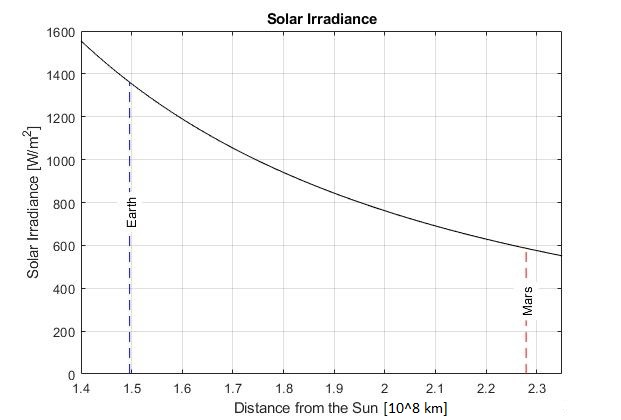
\includegraphics[width=0.7\textwidth]
    {Pictures/solar_irradiance.jpg}
    \caption{Solar irradiance during the mission as a function of distance from the Sun}
    \label{picture_solar_irradiance}
\end{figure}

\noindent When the spacecraft has started to orbit Mars the spacecraft is sometimes in eclipse and solar panels cannot produce power. During eclipse the spacecraft must rely on batteries. When the spacecraft is not in eclipse the solar panels receive a solar irradiance with an average value of $586.2W/m^2$. The time spacecraft spends in sunlight and in eclipse during one orbit around the planet depends on the angle $\alpha$ between sun rays and the orbital plane of the spacecraft ($\alpha$ in Figure \ref{picture_mars_seasons}). As the Martian year proceeds the angle $\alpha$ changes. From Figure \ref{picture_mars_seasons} it can be seen that when the mentioned angle is $0^{\circ}$ the time spacecraft spends in eclipse is the longest. When the mentioned angle is $90^{\circ}$ the spacecraft does not enter the eclipse at all during its orbital period. Eclipse time study was done with Matlab simulation and the result of the simulation is shown in Figure \ref{picture_eclipse_duration} which presents the durations the spacecraft spends in sunlight and in eclipse in different phases of the mission during one orbit around Mars. From the mentioned figure it can be seen that the longest continuous time spacecraft would spend in eclipse would be $41min$. It can also be observed that the spacecraft has periods when it does not enter the eclipse at all during its orbit. These periods last $0.32$ Earth years and happen every $0.94$ Earth years.\\

\begin{figure}[H]
	\centering 
	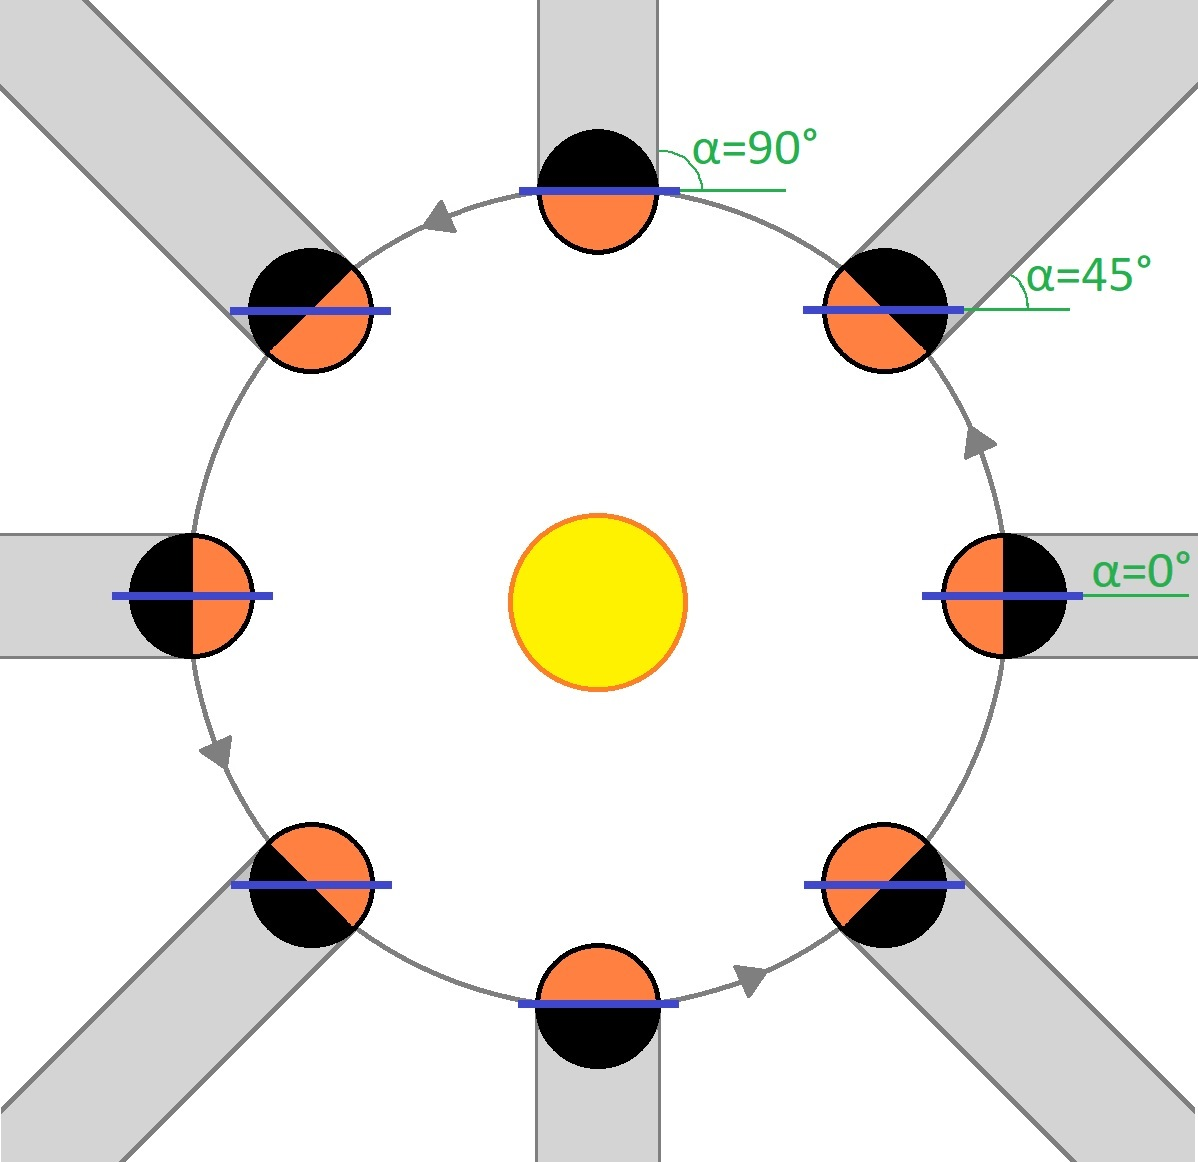
\includegraphics[width=0.5\textwidth]
    {Pictures/mars_seasons.jpg}
    \caption{Sketch showing how the angle between sun rays and the orbital plane changes during a Martian year. Sketch shows Mars in 8 different positions around the Sun during a Martian year (1.881 Earth years \cite{Mars Fact Sheet}). Blue line represents the orbit of the spacecraft around Mars.}
    \label{picture_mars_seasons}
\end{figure}

\begin{figure}[H]
	\centering 
	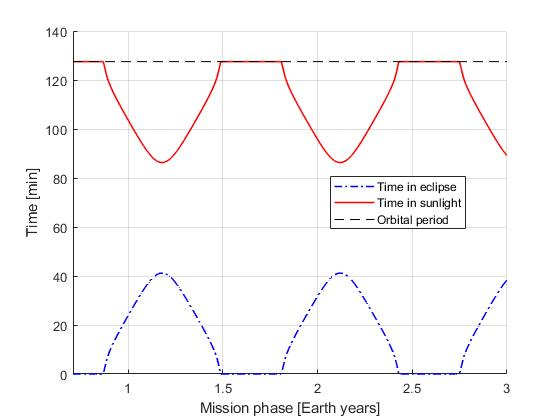
\includegraphics[width=0.7\textwidth]
    {Pictures/eclipse_duration.jpg}
    \caption{Time span the spacecraft would spend in eclipse and in sunlight during single orbit around Mars in different phases of the mission.}
    \label{picture_eclipse_duration}
\end{figure}

The following assumptions were made during the study of eclipse duration.
\begin{itemize}
\item Circular Martian orbit
\item The orbital plane of the spacecraft is perpendicular to Mars orbit around the Sun (i.e. a perfect polar orbit with inclination of $90^{\circ}$).
\item Time of the spacecraft spends in Mars' penumbra is considered to be negligible and the border of Mars' umbra is parallel with sun rays (i.e. hard shadow assumption)
\item The direction of the orbital plane of the spacecraft is fixed and oblateness effect is disregarded. 
\end{itemize}

\noindent The battery system forming the secondary power source could be designed, when the maximum eclipse time and seasons where the spacecraft would be all the time in sunlight were determined. The power needed for charging the batteries could be defined giving the maximum power needed from the solar panels setting the limit for panel dimensioning. The solar cell used is a "Triple Junction Solar Cell 3G30C-Advanced (BOL)" manufactured by Azur space \cite{Solar_cell}. This cell was chosen because of its light weight, high efficiency and company's high number of reference missions. The characteristics of the mentioned cell are given by the manufacturer and are presented in Table \ref{table_solar_cell}.\\

% Table containing single cell properties Here
\begin{table}[h]
 \caption{Characteristics for "Triple Junction Solar Cell 3G30C-Advanced (BOL)" solar cell by Azur Space when irradiance is $1367W/m^2$ and temperature is $28^{\circ}C$ \cite{Solar_cell}}
 \label{table_solar_cell}
\centering
 \begin{tabular}{| c | c |}
  \hline
	\textbf{Physical}	& \\
  \hline
  	Width [$mm$]		& 40.15 \\
    Length [$mm$]		& 80.15 \\
    Thickness [$mm$]	& 0.28 \\
    Absorptivity coefficient & $\leq$ 0.91\\
  \hline
  	\textbf{Electrical} & \\
  \hline
  	Voltage at max power [$V$] & 2.409\\
    Current at max power [$A$] & 0.5029\\
    Average efficiency & 0.293\\
    Power degradation [$\%/year$] & 5\\
  \hline
  	\textbf{Temperature gradients} & \\
  \hline
  	Voltage at max power [$V/^{\circ}C$] & -0.0067\\
    Current at max power [$A/^{\circ}C$] & +0.00024\\
  \hline
\end{tabular}
\end{table}

A rough estimation about solar panel temperature in different parts of the mission was performed with Stefan-Boltzmann law described with Equation \ref{equation_Stefan_Boltzmann}. 

\begin{equation}
T=\Bigg(\frac{I_x\alpha-P/A}{\sigma\varepsilon}\Bigg)^{1/4}
\label{equation_Stefan_Boltzmann}
\end{equation}

In this equation $I_x$ is the solar irradiance in the location of the spacecraft, $\alpha$ is the absorptivity coefficient of the solar panels, $P/A$ is the electrical power produced by the solar panels per panel area, $\sigma$ is the Boltzmann constant having the value of $5.670373*10^{-8}$ and $\varepsilon$ is the emissivity of the solar panels. According to solar cell datasheet absorptivity coefficient $\alpha$ gets values in the range of $\leq 0.91$ and the value $\alpha=0.91$ was chosen for this study \cite{Solar_cell}. Emissivity coefficient was estimated to be $\varepsilon=0.85$, typical magnitude for advanced triple junction solar cell which is used in this design \cite{Solar_cell_emissivity}. The results of the temperature estimations for the solar panels in different parts of the mission are presented in Table \ref{table_solar_panel}.\\

\noindent The solar panel configuration is designed assuming the worst case conditions i.e. the conditions where the power production in sunlight is the smallest. These conditions are present at the end of the mission when the degradation of the solar panels has continued the longest amount of time due to the radiation effects and the spacecraft is orbiting Mars where the solar irradiance is the lowest during the mission. %Even though the solar panel efficiency is lowest when leaving Earth due to high temperature of the panels, the low solar irradiance at the orbit around Mars makes the power production smallest at the end of the mission. Also the degradation of the solar panels due to radiation effects has continued longest amount of time at the end of the mission resulting to efficiency and supply power decrease between the time when spacecraft arrives to Mars and the mission ends.
Taking these effects into account the solar panel configuration was designed so that they would produce the required $600W$ of power at the voltage level of about $28V$ always when the spacecraft is in sunlight. The characteristics of the resulting solar panel design are presented in Table \ref{table_solar_panel}.\\

\noindent Table \ref{table_solar_panel} also describes how the solar panels perform in different phases of the mission. When the spacecraft starts the mission and is near Earth, solar panels produce much more power than near Mars where the solar irradiance is considerably smaller. From the table it can be seen that the power produced is larger when the spacecraft arrives to Mars than what it is when the mission ends. The difference is caused by power degradation due to radiative effects on the solar cells. Important thing worth noting is that solar panels produce a considerable amount of excess power during every part of the mission forming a power buffer. The buffer brings several advantages to the power system. First of all solar panels are allowed to diverge from $0^{\circ}$ incident light angle meaning that attitude corrections are not needed that frequently. Secondly, loss of few solar cells is tolerated (buffer size is equal to the worst case power production of 56 cells) as well as other unexpected malfunctions on-board (e.g. short circuits, resistance increase in components due to radiative effects etc.). Lastly, solar panels can be used outside the maximum power point. This is crucial characteristic when the spacecraft is leaving Earth. In Table \ref{table_solar_panel} the voltage level when leaving LEO is only $25.3V$ - too small to supply $28V$ power bus. However $25.3V$ is the voltage for maximum power point where the excess power is $817.8W$. Because of this the solar cells can be operated at sufficiently large voltage with produced power being slightly smaller.

% Table containing solar panel characteristics
\begin{table}[H]
 \caption{Characteristics of the spacecraft solar panel in different phases of the mission}
 \label{table_solar_panel}
\centering
 \begin{tabular}{| >{\centering\arraybackslash}p{5.9cm} | >{\centering\arraybackslash}p{2.9cm} | >{\centering\arraybackslash}p{2.9cm} | >{\centering\arraybackslash}p{2.9cm} |}
  \hline
	\textbf{Configuration properties}	& Leaving LEO $t=0.00$ $years$ & Arriving to Mars $t=0.72$ $years$ & Mission end $t=3.00$ $years$ \\
  \hline
  	Cells in series		& 13 & Same & Same   \\
    Cells in parallel	& 108 & Same & Same   \\
    Cell amount & 1404 & Same & Same \\
    Mass [$kg$]	& 5.33 & Same & Same   \\
    Area [$m^2$] & 4.52 & Same & Same  \\
  \hline
  	\textbf{Environment conditions} &  &  &  \\
  \hline
  	Temperature [$^{\circ}C$] & $97.5$ & $22.2$ & $26.5$  \\
    Solar irradiance [$W/m^2$] & 1367.0 & 588.9 & 588.9  \\
  \hline
  	\textbf{Electrical properties} &  &  &   \\
  \hline
  	Efficiency & 0.245 & 0.287 & 0.250 \\
  	Supply voltage [$V$] & 25.3 & 31.3 & 29.0 \\
    Supply current [$A$] & 56.1 & 22.9 & 21.6 \\
    Supply power [$W$] & 1417.8 & 716.2 & 625.1 \\
    Excess power [$W$] & 817.8 & 116.2 & 25.1 \\
    Power per panel unit mass [$W/kg$] & 265.9 & 134.3 & 117.2 \\
  \hline
\end{tabular}
\end{table}

\noindent The following assumptions were made during the design study of solar panels.
\begin{itemize}
\item Degradation happens at constant rate of $5\%/year$ during the entire mission \cite{Solar_panel_degradation}
\item Radiative power of the Sun follows a long term average value and remains constant.
\item Sun is considered as a point source radiator
\item Solar cells operate at their maximum power point. Shunt voltage limiter is able to consume the excess power and voltage regulation keeps the voltage at about $28V$
\item A control on the gimble makes sure the solar panels are facing the Sun constantly with a decided angle from ground control.
\item All the solar cells produce power simultaneously, meaning that there is no mismatch between them.
\item Solar panel temperature is affected only by direct sunlight and temperature change due to exiting and entering eclipse is neglected. These assumptions are coarse but extensive research including reflections from Earth and Mars and effect of changing illumination conditions are outside of the scope of this study.
\end{itemize}

\subsubsection{Batteries}

Batteries are intended to provide power when solar panels are not in use, that is during launch and eclipses around Mars. The scaling of the battery will only take into account the power needed during the eclipses. It can be assumed that the satellite will be hit by sunlight all along its cruise between earth and mars. The solar panels will provide the required power during this phase. During the eclipses around mars, batteries will take over before the satellite reaches sunlight again. They will then be recharged. 
 %verify the power consumption to heat up the satellite \\
The continuous maximum power required during the eclipse time is fixed at 55 Watts in a conservative way, which represents roughly the total energy of 37.6 Wh for the longest eclipse duration of 41 minutes. This energy will mainly be used occasionally during the attitude control maneuvers.

The batteries chosen for this mission are cylindrical lithium-ion cells, known for their high specific energy, in this case 154 Wh/Kg. The charging of those batteries requires a suitable regulation of the voltage and current delivered from the solar panels. A charge circuit is provided by the manufacturer, above the battery pack. The main characteristics of the Li-ion cells chosen are summed up in Table \ref{Li-ion_cell_characteristics}. Those data are inspired by GomSpace Li-ion 1850 battery pack, used for space applications \cite{Lithium Ion 18650 cells for space flight products datasheet}.

% \begin{table}[H]
% \centering
% \caption{GomSpace Lithium-ion cell 18650 main characteristics}
% \label{Li-ion_cell_characteristics}
% \begin{tabular}{|c|c|}
% \hline
% \multicolumn{2}{|c|}{\textbf{BATTERY CELL}}     \\ \hline
% \textbf{Battery type}                  & Li-ion \\ \hline
% \textbf{Cell voltage (V)}              & 3.7    \\ \hline
% \textbf{Cell capacity (Ah)}            & 2.6    \\ \hline
% \textbf{Energy (Wh)}                   & 9.6    \\ \hline
% \textbf{Height (mm)}                   & 65     \\ \hline
% \textbf{Diameter (mm)}                 & 18.5   \\ \hline
% \textbf{Volume (cm\textasciicircum 3)} & 17.5   \\ \hline
% \textbf{Weight (g)}                    & 48     \\ \hline

% \end{tabular}
% \end{table}

\begin{table}[h]
 \caption{GomSpace Lithium-ion cell 18650 main characteristics}
 \label{Li-ion_cell_characteristics}
\centering
 \begin{tabular}{| c | c |}
  \hline
	\multicolumn{2}{|c|}{\textbf{BATTERY CELL}}     \\
  \hline
  	Battery type		& Li-ion \\
    Cell voltage [$V$]  & 3.7  \\
    Cell capacity [$Ah$]& 2.6 \\
    Energy [$Wh$]       & 9.6 \\
    Height [$mm$]       & 65 \\
    Diameter [$mm$]     & 18.5 \\
    Volume [$cm^{3}$]       & 17.5 \\
    Weight [$g$]       & 48 \\
  \hline
\end{tabular}
\end{table}

The chosen voltage at the battery is 29.6 V, a common used voltage for space applications. The battery packs will contain 8 cells in series, according to the 8S-1P configuration from the manufacturer \cite{Hi-capacity battery pack for nano satellites datasheet}. The required capacity depends on the lifetime needed for the mission. Assuming that the satellite will orbit during 2.3 years around mars, the batteries will have to make a maximum of 6242 cycles, discharging during a time comprised between a few seconds and 41 minutes. For safety reasons, all the cycles are assumed to last 41 minutes. By choosing a low Depth Of Discharge, the lifetime of the battery is extended. According to the manufacturer's data \cite{Lithium Ion 18650 cells for space flight products datasheet}, a DOD of 6.1\% ensures a long enough lifetime, assuming that dividing the DOD by 2 leads to a 2 times longer lifetime. The capacity loss is given at 5\% per year. Thus, the required battery pack characteristics are presented in Table \ref{Battery_pack}. 

% \begin{table}[H]
% \centering
% \caption{Battery packs characteristics}
% \label{Battery_pack}
% \begin{tabular}{cc}
% \hline
% \multicolumn{2}{|c|}{\textbf{BATTERY PACKS}}                                                     \\ \hline
% \multicolumn{1}{|c|}{\textbf{Pack configuration}}                  & \multicolumn{1}{c|}{8S-1P} \\ \hline
% \multicolumn{1}{|c|}{\textbf{Voltage (V)}}                         & \multicolumn{1}{c|}{29.6}  \\ \hline
% \multicolumn{1}{|c|}{\textbf{Capacity (Ah)}}                       & \multicolumn{1}{c|}{20.8} \\ \hline
% \multicolumn{1}{|c|}{\textbf{Number of cells in series}}           & \multicolumn{1}{c|}{8}     \\ \hline
% \multicolumn{1}{|c|}{\textbf{Number of cells parallel}}            & \multicolumn{1}{c|}{8}     \\ \hline
% \multicolumn{1}{|c|}{\textbf{Number of battery packs}}             & \multicolumn{1}{c|}{8}     \\ \hline
% \multicolumn{1}{|c|}{\textbf{Total number of cells}}               & \multicolumn{1}{c|}{64}    \\ \hline
% \multicolumn{1}{|c|}{\textbf{Total volume (dm\textasciicircum 3)}} & \multicolumn{1}{c|}{2.623} \\ \hline
% \multicolumn{1}{|c|}{\textbf{Total weight (kg)}}                   & \multicolumn{1}{c|}{4}     \\ \hline
% \multicolumn{1}{|c|}{\textbf{Power dissipation (W)}}               & \multicolumn{1}{c|}{4.48}  \\ \hline
% \multicolumn{1}{l}{}                                               & \multicolumn{1}{l}{}      
% \end{tabular}
% \end{table}

\begin{table}[h]
 \caption{Battery packs characteristics}
 \label{Battery_pack}
\centering
 \begin{tabular}{| c | c |}
  \hline
	\multicolumn{2}{|c|}{\textbf{BATTERY PACKS}}     \\
  \hline
  	Pack configuration		& 8S-1P \\
    Nominal voltage [$V$]   & 29.6  \\
    Nominal capacity [$Ah$] & 20.8 \\
    Number of cells in series           & 8 \\
    Number of cells in parallel & 8 \\
    Number of battery packs & 8 \\
    Total number of cells & 64 \\
    Total volume [$dm^{3}$]       & 2.623 \\
    Total weight [$kg$]         & 4 \\
    Power dissipation [$W$]     & 5.5 \\
  \hline
\end{tabular}
\end{table}


The maximum charging time at 0.1C is estimated at 37 minutes with a DOD of 6.1\%. The battery has enough time to recharge even during the shortest light period. The voltage should remain between 3 and 4.2 V for each cell. During charging, the temperature of the batteries should remain between 0 and 45 degrees Celsius and between -20 and 60 degrees Celsius when discharging. The lifetime of the battery is estimated at 7000 cycles which represents 2 earth years and 7 months. The power dissipation in heat from the battery is estimated at 10\% of its total power. The low DOD leads to a quite high "dead mass" of the batteries, but the final weight of 4 kg is worth it.

\subsection{Propulsion system}
The Mass Orbiter Mission (MOM) is considered for inspiration in the propulsion system choice due to use of the same payload \cite{MOM}. Two propulsion systems are used for this mission. One main engine of 440N thrust and mass of 4.3kg to send the satellite from Earth to Mars and eight small thrusters of 22N and mass of 0.8kg each for attitude control. The propellant used is a bi-propellant consisting of monomethylhydrazine (MMH) and dinitrogen tetroxide (N$_{2}$ O$_{4}$). 

The rocket equation is used to estimate the mass of the propellant required.
\begin{equation}
\label{racket}
\Delta v = I_{sp}*g*\ln\frac{m_{wet}}{m_{dry}}
\end{equation}
where,
\begin{equation}
\label{propmass}
m_{wet} = m_{dry} + m_{prop}
\end{equation}

The mass of the propellant is calculated around 960 kg. As a safety factor, a total mass of about 1-1.1 tonnes of propellant is used to account for attitude control maneuvers. Two pressurized tanks are used, one for the propellant and one for the oxidizer, with an estimated volume of 400L and a mass of 35kg each, similar to MOM mission. Finally, the dry mass of the satellite is estimated about 250 kg, summing up all the components' mass of the satellite .


\section{Thermal System}

\subsection{ Thermal model }

A thermal simulation has been realized using the Thermica software for the satellite. The satellite is modeled by a cube with solar panels whose dimensions are in Table \ref{dimensions}. It is assumed that there are equipments and radiators on four of the six faces of the cube. The choice of placing equipments on only four of the faces was motivated by constraints of the model used in Thermica that was available for this study.

\begin{table}[H]
 \caption{Dimensions of the satellite}
 \label{dimensions}
\centering \begin{tabular}{| c | c |c |}
  \hline
 &  Cube & Solar panels  \\
   \hline
 Width & 1.5 m & 1 m     \\
     \hline
 Length & 1.5 m & 4 m    \\
     \hline
\end{tabular}
\end{table}

The equipments are assumed to be mounted on each surface with a connection node with the conductivity 40 J/K. Each radiator is made with SSM aluminum which has an absorption coefficient of 0.15  at the beginning of its life (BOL) and 0.19 in the end of life (EOL). The emissivity coefficient is 0.78. Beside a radiator, each surface is covered with multilayer insulator (MLI). 

\medskip

Equipment have been placed on the faces of the satellite according to the requirements of the mission. Their places are detailed in Table \ref{places}. Only the solar panels have been modeled in Thermica as can be seen in Figure \ref{model}. -Y is pointing to Mars and the velocity of the satellite is parallel to +Z. Radiators will be placed on -Y, +Y, -Z and +Z.

\begin{table}[H]
 \caption{Place of the equipment on the different surfaces of the satellite.}
 \label{places}
\centering \begin{tabular}{| c | c |c |c |c |c |c |}
  \hline
Face & +X & -X & +Y & -Y & +Z & -Z\\
   \hline
 Equipment & Solar panel & Thruster  & Telemetry & Camera & Part of the tanks & / \\
     \hline
\end{tabular}
\end{table}

\begin{figure}[H] 
\centering
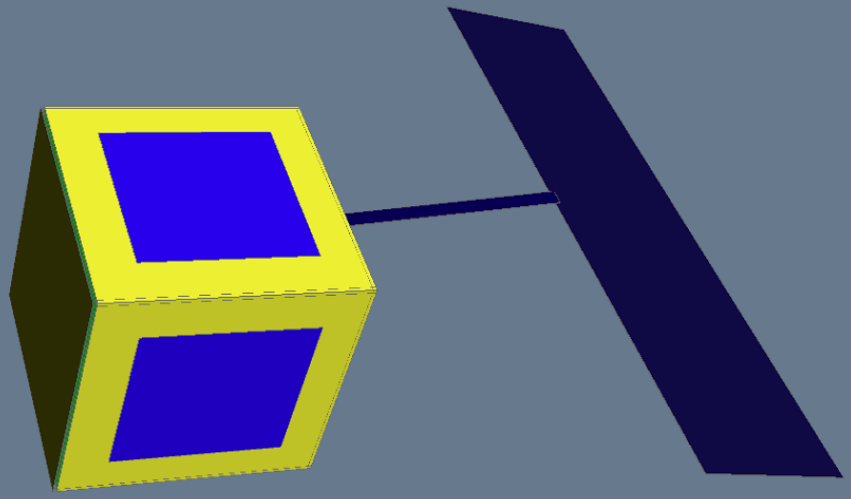
\includegraphics[scale=0.38]{model.png}
\caption{Model of the satellite on Thermica.}
\label{model}
\end{figure}


For this thermal simulation, a sun-synchronous orbit was chosen, rather than a polar one. Sun-synchronous orbits are indeed the best for observation of planets considering that they allow to keep a constant sunlight. Studying a polar orbit was nevertheless more interesting for the other parts of this project considering the fact that it implies more constraints and requirements.

\medskip

With this sun-synchronous orbit, the simulation has been done in two different thermal cases which represent the extreme conditions that the satellite will encounter around Mars. Considering its elliptical orbit, Mars is closer to the Sun during the northern winter than in summer. It means that the two cases are:
\begin{itemize}
    \item \textbf{Cold case:} Mars at aphelion in beginning of life (BOL): simulated on October 7, 2017. In this case the satellite receives little energy and material are still efficient.
    \item \textbf{Hot case:} Mars at perihelion in end of life (EOL): simulated on September 16, 2018. In this case the satellite receives lot of energy and material are less efficient.
\end{itemize}

\subsection{ Net thermal flux}

\medskip

The absorbed flux of each surface $M_a$ can be calculated with Equation \ref{absorbed}

\begin{equation}
\fbox{$M_a=M_{sun}+M_{MAlbedo}+M_{MIR}$}
\label{absorbed}
\end{equation}

where $M_{sun}$ is the absorbed flux due to the sun thermal flux, $M_{MAlbedo}$ due to the Mars albedo and $M_{MIR}$ due to the Mars infrared flux. These three absorbed flux have been calculated in Thermica and are shown in Tables \ref{AbsorbedCold}, \ref{AbsorbedHot}. 

\begin{table}[!h]
 \caption{Absorbed flux in cold case ($\text{W/m}^\text{2}$).}
 \label{AbsorbedCold}
\centering \begin{tabular}{| c | c |c |c |c |}
  \hline
Face &  $\text{M}_\text{{sun}}$ & $\text{M}_\text{{MAlbedo}}$ & $\text{M}_\text{{MIR}}$ & $\text{M}_\text{a}$ \\
   \hline
+Y & 22.5  & 0 & 0 & 22.5 \\
   \hline
-Y & 3.5  & 2.6 & 93.7 & 99.8 \\
   \hline
+Z & 0  & 0.6 & 22.2 & 22.8 \\
   \hline
-Z &  15.6 &  0.7 & 24.6 & 40.9 \\
   \hline
\end{tabular}
\end{table}

\begin{table}[!h]
 \caption{Absorbed flux in hot case ($\text{W/m}^\text{2}$).}
 \label{AbsorbedHot}
\centering \begin{tabular}{| c | c |c |c |c |}
  \hline
Face &  $\text{M}_\text{{sun}}$ & $\text{M}_\text{{MAlbedo}}$& $\text{M}_\text{{MIR}}$ & $\text{M}_\text{a}$  \\
\hline
+Y & 40.8 & 0 & 0 & 40.8 \\
     \hline
-Y & 7.3	 & 4.7	 & 93  & 105  \\
     \hline
+Z & 0 & 1 & 21.8 & 22.8 \\
     \hline
-Z & 33.3 & 1.3& 24.6 & 59.2\\
     \hline
\end{tabular}
\end{table}


Assuming that the radiators can be considered as gray bodies the emitted flux of a surface can be calculated with Equation \ref{emitted}.

\begin{equation}
\fbox{$M_e=\epsilon*\sigma*T^4$}
\label{emitted}
\end{equation}

where T is the temperature of the radiator in kelvin and $\sigma$ is the Stefan Boltzmann's constant. T is considered to be $5^{\circ}$C in the cold case and $20^{\circ}$C in the hot case.

In the end, the net thermal flux per unit surface is given by Equation \ref{net}.

\begin{equation}
\fbox{$M=M_e-M_a$}
\label{net}
\end{equation}

The calculations give the results in Table \ref{netTable}.

\begin{table}[H]
 \caption{Net thermal flux per unit surface ($\text{W/m}^\text{2}$).}
 \label{netTable}
\centering \begin{tabular}{| c | c |c |c |c |c |c |}
  \hline
Face &  +Y & -Y & +Z & -Z \\
     \hline
Net Flux Cold Case ($\text{W/m}^\text{2}$) & 223 & 146 & 223  & 205 \\
     \hline
 Net Flux Hot Case ($\text{W/m}^\text{2}$) & 285 & 221 &  303 &  267 \\
     \hline
\end{tabular}
\end{table}

Considering these results and their dissipated power ADCS is placed on +Y, On Board Computer (OBC) is placed on -Y and the batteries are placed on +Z. 

The final configuration of the equipment is then the one described in Table \ref{finalPlaces}.



\begin{table}[!h]
 \caption{Final places of the equipment on the different surfaces of the satellite, masses and dissipated powers.}
 \label{finalPlaces}
\centering \begin{tabular}{| c | c |c |c |c |c |c |}
  \hline
Face & +Y & -Y & +Z & -Z\\
   \hline
 Equipment  & Telemetry+OBC & Camera &  Tank+ADCS  & Batteries\\
     \hline
 Hot case dissipation (W)  & 18.2 + 15 &  3.5 & /+112 & 4.5  \\
     \hline
Cold case dissipation (W)  & 0 + 10 & 3.5 & /+50 & 1  \\
     \hline
Mass (kg)  & 4.9 + 5 & 5 & /+30 & 4  \\
     \hline
\end{tabular}
\end{table}

\subsection{Radiators}

Assuming that the radiators temperature should remain below $20^{\circ}$C, the area of the radiators can be determined by writing the thermal equilibrium as in Equation \ref{areaE}.

\begin{equation}
\fbox{$A=\frac{P_d}{\epsilon*\sigma*T^4-M_a}$}
\label{areaE}
\end{equation}

where $P_d$ is the power dissipated.

Using the values for the hot case of Table \ref{AbsorbedHot} and Table \ref{finalPlaces} for the dissipation, the radiators should have the areas written in Table \ref{areaT}.

\begin{table}[!h]
 \caption{Minimum areas for the radiators in order to keep the temperature below $20^{\circ}$C.}
 \label{areaT}
\centering \begin{tabular}{| c | c |c |c |c |}
  \hline
Face & +Y &  -Y  & +Z & -Z  \\   
   \hline
 Radiator area ($\text{m}^\text{2}$) & 0.12 & 0.016  & 0.37 &  0.017 \\
     \hline
\end{tabular}
\end{table}

\subsection{Results}

\subsubsection{Temperatures in the hot case}

The temperature that each radiator on each face of the satellite would have during 20 orbits around Mars has been simulated with Thermica in the hot case using the radiators of Table \ref{areaT}. In this simulation, internal radiations were taken into account. 
To optimize the results, considering that the calculations of the areas were not based on the internal radiations, these areas have then be adjusted to get more satisfying temperatures. In the end the optimized areas are the ones in Table \ref{areaTOpt}.

\begin{table}[!h]
 \caption{Optimized minimum areas for the radiators.}
 \label{areaTOpt}
\centering \begin{tabular}{| c | c |c |c |c |}
  \hline
Face & +Y &  -Y  & +Z & -Z  \\   
   \hline
 Radiator area ($\text{m}^\text{2}$) & 0.06 & 0.008  & 0.22 &  0.008 \\
     \hline
\end{tabular}
\end{table}

The temperatures of each radiators during 20 orbits around Mars are represented in Figure \ref{tempPYHOT}, \ref{tempMYhot}, \ref{tempPZHOT} and \ref{tempNZhot}. The temperature remains always between $-1^{\circ}$C and $18^{\circ}$C.

\begin{figure}[!ht] 
\begin{minipage}{8cm}
\centering
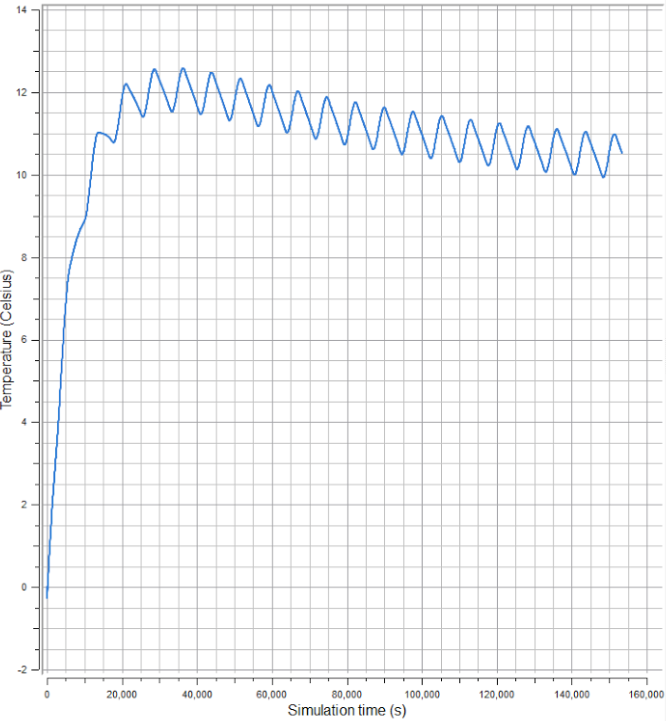
\includegraphics[scale=0.38]{PYhot}
\centering
\caption{Temperature of the +Y radiator in the hot case with respect to the time, during 20 orbits around Mars.}
\label{tempPYHOT}
\end{minipage} 
\medskip
\begin{minipage}{8cm}
\centering
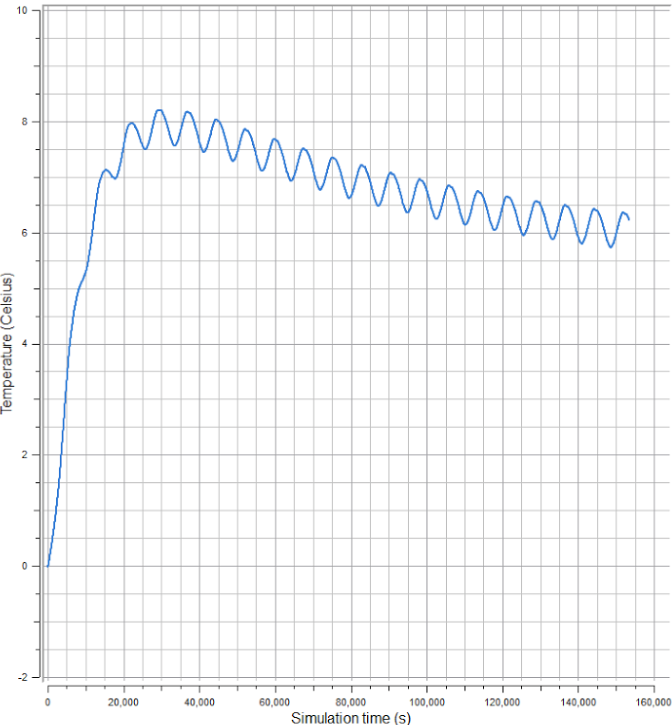
\includegraphics[scale=0.39]{NYhot}
\caption{Temperature of the -Y radiator in the hot case with respect to the time, during 20 orbits around Mars.}
\label{tempMYhot}
\end{minipage} 
\end{figure}

\begin{figure}[!ht] 
\begin{minipage}{8cm}
\centering
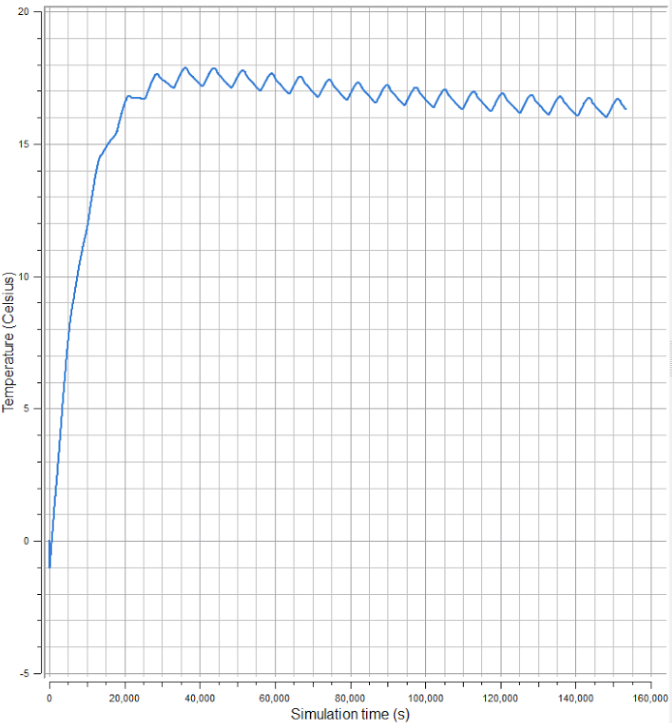
\includegraphics[scale=0.37]{PZhot}
\centering
\caption{Temperature of the +Z radiator in the hot case with respect to the time, during 20 orbits around Mars.}
\label{tempPZHOT}
\end{minipage} 
\medskip
\begin{minipage}{8cm}
\centering
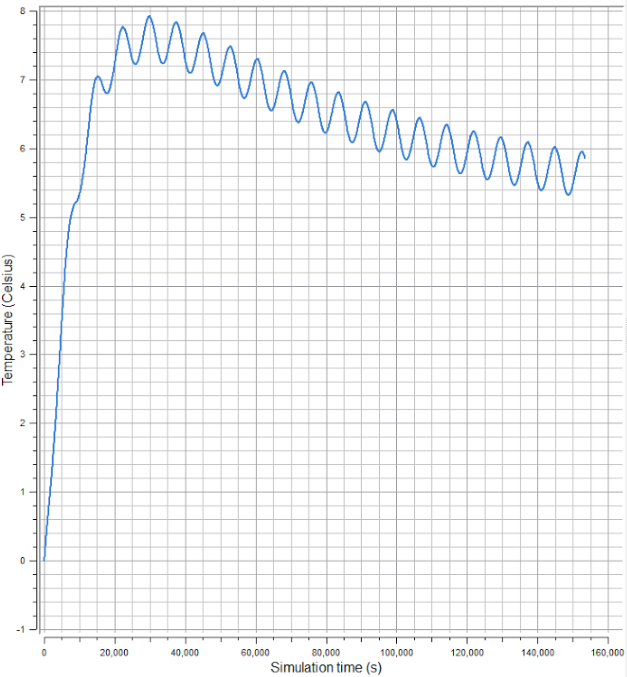
\includegraphics[scale=0.38]{NZhot}
\caption{Temperature of the -Z radiator in the hot case with respect to the time.}
\label{tempNZhot}
\end{minipage} 
\end{figure}


\subsection{Heaters}

In order to keep the temperature upon $5^{\circ}$C, heaters can be placed on each face. Their power can be determined with Equation \ref{heaterE}.

\begin{equation}
\fbox{$M_H= A*\epsilon*\sigma*T^4-A*M_a-P_d$}
\label{heaterE}
\end{equation}

where $M_H$ is the power of the heater, A the area of the optimized radiator. 

With $T=5^{\circ}$C in the cold case and using the values for the cold case of Table \ref{AbsorbedCold} and Table \ref{finalPlaces}, the heaters should have the power written in Table \ref{heaterT}. A negative value in this table means that no heater is necessary on the face.

\begin{table}[!h]
 \caption{Minimum power for the heaters in order to keep the temperature upon $5^{\circ}$C.}
 \label{heaterT}
\centering 
\begin{tabular}{| c | c |c |c |c |}
  \hline
Face & +Y &  -Y  & +Z & -Z  \\
   \hline
 Heater power (W) & 4.5 & -2.2 & 3.1  & 0.79\\
     \hline
\end{tabular}
\end{table}


\subsubsection{Temperatures in the cold case}

As for the hot case, the temperature that each face of the satellite would have during 20 orbits around Mars has been simulated with Thermica in the cold case using the radiators of Table \ref{areaTOpt} and the heaters of Table \ref{heaterT}. In this simulation, heaters are activated when the temperature is below $0^{\circ}$C and deactivated when the temperature is upon $5^{\circ}$C.

As for the radiators areas, the heaters powers have then be optimized to get the most satisfying temperatures. The results of the optimization are shown in Table \ref{heaterTopti}. 

\begin{table}[H]
 \caption{Optimized minimum power for the heaters.}
 \label{heaterTopti}
\centering 
\begin{tabular}{| c | c |c |c |c |}
  \hline
Face & +Y &  -Y  & +Z & -Z  \\
   \hline
 Heater power (W) & 4.5 & 2.5 & 3.1  & 2.5\\
     \hline
\end{tabular}
\end{table}


The temperatures of each faces during 20 orbits around Mars are represented in Figure \ref{tempPYcold}, \ref{tempNYcold}, \ref{tempPZcold} and \ref{tempNZcoldT}. The temperature remains always between $-1^{\circ}$C and $13^{\circ}$C. In Figure \ref{tempPZcold}, the activation of the heater can be seen in the beginning of the simulation, when the temperature drops to $-1^{\circ}$C.

\begin{figure}[!ht] 
\begin{minipage}{8cm}
\centering
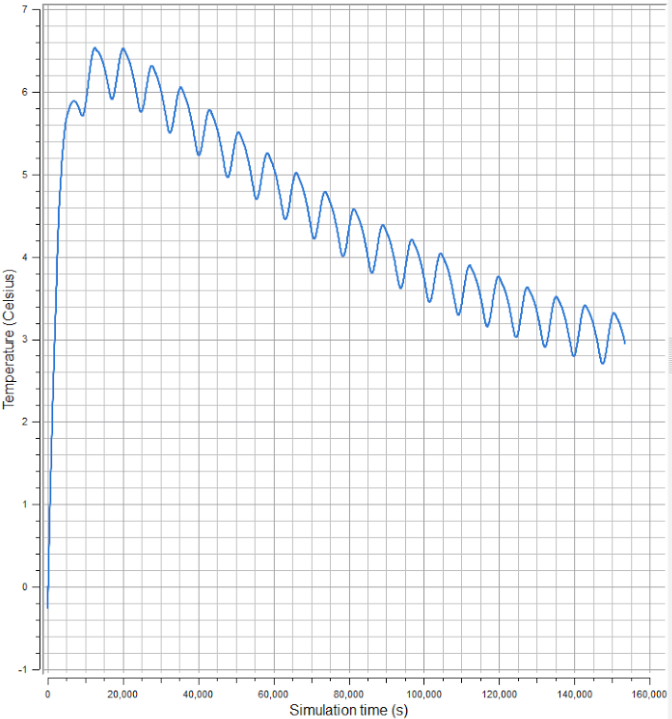
\includegraphics[scale=0.38]{PYcold}
\centering
\caption{Temperature of the +Y radiator in the cold case with respect to the time.}
\label{tempPYcold}
\end{minipage} 
\medskip
\begin{minipage}{8cm}
\centering
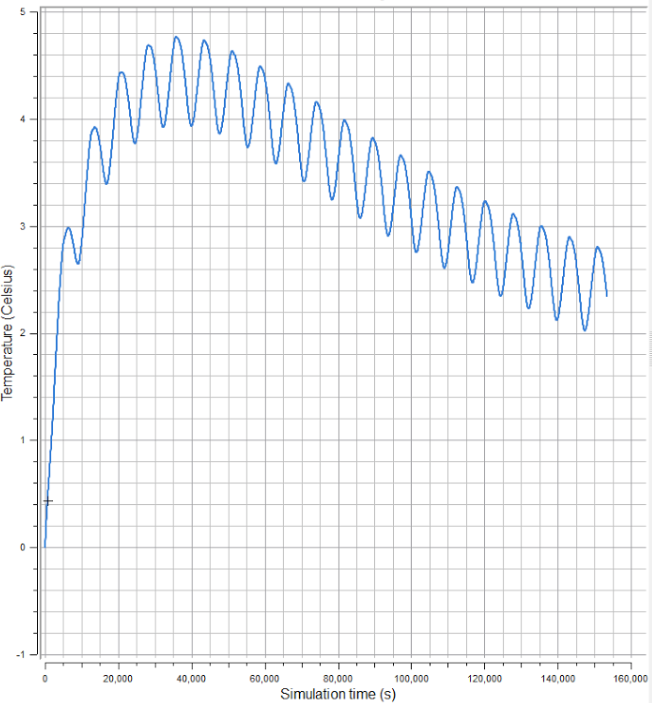
\includegraphics[scale=0.39]{NYcold}
\caption{Temperature of the -Y radiator in the cold case with respect to the time.}
\label{tempNYcold}
\end{minipage} 
\end{figure}

\begin{figure}[!ht] 
\begin{minipage}{8cm}
\centering
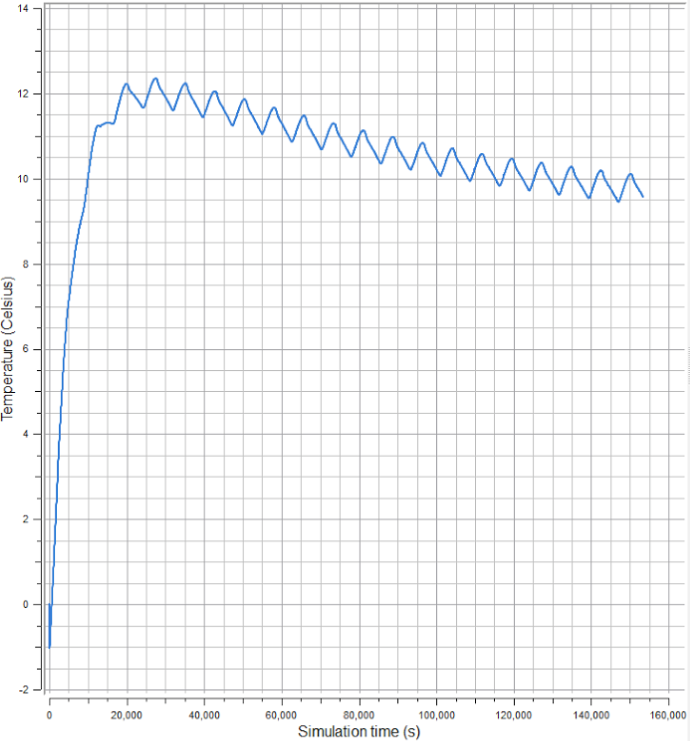
\includegraphics[scale=0.36]{PZcold}
\centering
\caption{Temperature of the +Z radiator in the cold case with respect to the time.}
\label{tempPZcold}
\end{minipage} 
\medskip
\begin{minipage}{8cm}
\centering
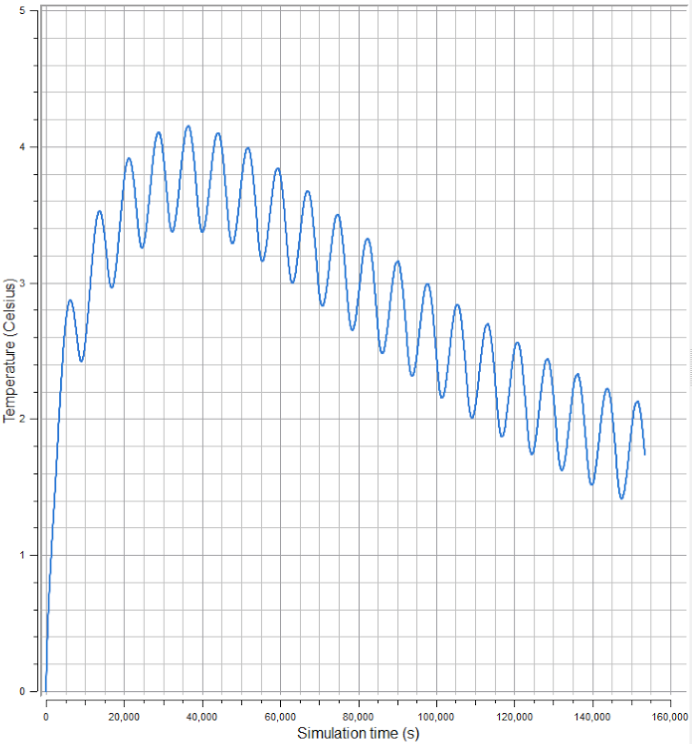
\includegraphics[scale=0.39]{NZcold}
\caption{Temperature of the -Z radiator in the cold case with respect to the time.}
\label{tempNZcoldT}
\end{minipage} 
\end{figure}

\clearpage

\section{Conclusions}

The feasibility study of a mission to Mars has been evaluated. More efforts have been put to Power system. A summary of relevant data is provided in Tables \ref{tab:tab1} and \ref{PS_charact}. \\
The total weight of the spacecraft at launch is 1.65 t (dry weight : 250 kg), it will send to earth 811 GB of data, therefore \textbf{the figure of merit is 503 MB/kg}.\\

\begin{table}[h]
\centering
\label{tab:tab1}
\caption{Weight and power consumption for each subsystem}
\begin{tabular}{| c | c | c |}
\hline
\textbf{Subsystem} & \textbf{Weight} [$Kg$] & \textbf{Max power consumption} [$W$] \\ \hline
AOCS & 30 & 450 \\ 
Telemetry & 4.9 & 68 \\ 
Camera & 5 & 5 \\ 
OBC & 5 & 0.6 \\ 
Thrusters & 11 & 35 \\ \hline

\end{tabular}
\label{tab:tab1}
\end{table}

\begin{table}[h]
\centering
\caption{Power systems main characteristics}
\label{PS_charact}
\begin{tabular}{ccc}
\hline
\multicolumn{1}{|c|}{\multirow{3}{*}{\textbf{Solar panels}}} & \multicolumn{1}{c|}{Output power [$W$]}     & \multicolumn{1}{c|}{625}   \\  
\multicolumn{1}{|c|}{}                                       & \multicolumn{1}{c|}{Area [$m^{2}$]}             & \multicolumn{1}{l|}{4.52}  \\ 
\multicolumn{1}{|c|}{}                                       & \multicolumn{1}{c|}{Weight [$kg$]}           & \multicolumn{1}{c|}{11}  \\ \hline
\multicolumn{1}{|c|}{\multirow{3}{*}{\textbf{Battery}}}      & \multicolumn{1}{c|}{Nominal capacity [$Ah$]} & \multicolumn{1}{c|}{20.8}  \\  
\multicolumn{1}{|c|}{}                                       & \multicolumn{1}{c|}{Volume [$dm^{3}$]}           & \multicolumn{1}{c|}{2.623} \\  
\multicolumn{1}{|c|}{}                                       & \multicolumn{1}{c|}{Weight [$kg$]}           & \multicolumn{1}{c|}{4}     \\ \hline
\multirow{2}{*}{}                                            &                                       &                            \\
                                                             &                                       &                            \\
\multirow{2}{*}{}                                            &                                       &                            \\
                                                             &                                       & \multicolumn{1}{l}{}       \\
\textbf{}                                                    &                                       & \multicolumn{1}{l}{}       \\
\multicolumn{1}{l}{}                                         & \multicolumn{1}{l}{}                  & \multicolumn{1}{l}{}      
\end{tabular}
\end{table}

In order to start with numerical data, two missions to Mars that occurred in the past, have been investigated. One from NASA called Mars Recoinnaissance Orbiter (MRO \cite{PaperMRO} and another from Indian space agency, called Mars Orbiter Mission (MOM \cite{MOM}). Also some data have been inspired by Trace gas Orbiter (TGO \cite{TGO}) mission from ESA.\\
Eventually, the data which have been sorted out for the design of this spacecraft are consistent with the previous missions.


\section{Division of work}

\begin{labeling}{workdivision}


\item [A. Cisowski] Worked on the Mission Analysis, telemetry, imagery

\item [R. Farid] Worked on the Payload and contributed to the solar panel design study.

\item [F.Giuliano] Worked on ADCS and collaborated to power system. He also wrote conclusions. Helped in reviewing. 

\item [J. Imbert] Worked on the Thermal System: estimation of radiators, heaters and satellite temperatures. Worked on the Mission Analysis.

\item [Y. Jiao] Worked on thermal simulation

\item [ C. Muresan] Worked on telemetry, imagery, preliminary battery and solar panel scaling.

\item [M. Nicolle] Was responsible for the study related to batteries and their scaling

\item [K. Papavramidis ] Worked on the Mission Analysis, Propulsion System and Power system. Responsible of reviewing everything. 

\item [S. Simolin] Was responsible of the study related to solar panels and their dimensioning

\item [F. Raiti] Choice of attitude determination sensors, estimation of reaction wheel power consumption, thermal simulation and estimation of radiator areas and heater powers.

\end{labeling}

\clearpage

\begin{thebibliography}{99}
\bibitem{Earth Fact Sheet}  NASA. (2016, 23 Dec). Earth Fact Sheet. Retrieved December 01, 2017, from 
https://nssdc.gsfc.nasa.gov/planetary/factsheet/earthfact.html.
\bibitem{MechanicsBook} Hill, P.; Peterson, C. (2010).  Mechanics and Thermodynamics of Propulsion
\bibitem{Mars Fact Sheet} NASA. (2016, 23 Dec). Mars Fact Sheet. Retrieved December 01, 2017, from nssdc.gsfc.nasa.gov/planetary/factsheet/marsfact.html.
\bibitem{PaperMRO} NASA, "Mars Reconnaissance Orbiter
Interplanetary Cruise Navigation", 20th International Symposium on Space Flight Dynamics
\bibitem{Power Systems Lecture EF2260} Lindqvist, P. (2017) Spacecraft Power Systems
\bibitem{Shunt voltage limiter} Teodorescu, M. (2013, May 24). Voltage Regulators: A Solar Panel's Riot Police. Retrieved December 01, 2017, from {https://www.electronicproducts.com/Power\$\_$Products/Power\$\_$Management/Voltage$\_$Regulators$\_$A$\_$Solar$\_$Panel$\_$39$\_$s$\_$Riot$\_$Police.aspx}
\bibitem{MOM} MARS ORBITER MISSION December 01, 2017 from https://www.isro.gov.in/pslv-c25-mars-orbiter-mission
\bibitem{Solar_cell}  Azur Space. (2016, August 19). 30\% Triple Junction GaAs Solar Cell Assembly - Type: TJ Solar Cell Assembly 3G30A. Retrieved December 02, 2017, from {http://www.azurspace.com/images/products/0003401-01-01$\_$DB$\_$3G30A.pdf}
\bibitem{TGO} Trace Gas Orbiter - \url{http://spaceflight101.com/exomars/trace-gas-orbiter/}
\bibitem{Lithium Ion 18650 cells for space flight products datasheet}  GomSpace. “Nano power battery : Lithium Ion 18650 cells” 2017, from
{https://gomspace.com/UserFiles/Subsystems/datasheet/gs-ds-nanopower-battery-16.pdf}
\bibitem{Hi-capacity battery pack for nano satellites datasheet}  GomSpace. “Nano power BSX : Hi-capacity battery pack for nano satellites datasheet” 2017, from
{https://gomspace.com/UserFiles/Subsystems/datasheet/gs-ds-nanopower-bpx-3-16.pdf}
\bibitem{Tanks} Bi-propellant tanks - \url{http://www.space-propulsion.com/spacecraft-propulsion/bipropellant-tanks/}
\bibitem{Tanks} Bipropellant Thrusters - \url{http://www.space-propulsion.com/spacecraft-propulsion/bipropellant-thrusters/}
 \bibitem{MarsCalendar} \url{http://www.planetary.org/explore/space-topics/mars/mars-calendar.html}
\bibitem{Solar_panel_degradation} NASA. (1971, 01 May). SPACECRAFT
SOLAR CELL ARRAYS. Retrieved December 05, 2017, from 
https://ntrs.nasa.gov/archive/nasa/casi.ntrs.nasa.gov/19710028154.pdf.
\bibitem{Solar_cell_emissivity} University of Leicester. (2008, December 03). CubeSat - The Technology Of Solar Cells. Retrieved December 05, 2017, from http://cubesat.wikidot.com/the-technology-of-solar-cells
\bibitem{Electra} The Electra Proximity Link Payload for Mars Relay TeIecommunications and Navigation Charles D. Edwards, Jr., Thomas C. Jedrey, Eric Schwartzbaum, and Ann S. Devereaux, Jet Propulsion Laboratory, Pasadena, CA 91 109, USA
 
\end{thebibliography}

\end{document}
